\documentclass{article}
\usepackage {color}
\usepackage {amsmath}
\usepackage {alltt}
\usepackage{graphicx} 
\usepackage{epstopdf}
\usepackage{caption} 
\usepackage{fancyvrb,relsize}
\usepackage[latin1]{inputenc}
\begin{document}

\title{Computing With Tiles}
\author{
Rahul Gopinath\\
gopinath@eecs.oregonstate.edu
\and
Yonglei Zheng\\
zheng@eecs.oregonstate.edu
\and
Madhura Vadvalkar\\
vadvalkar@eecs.oregonstate.edu
\and
Junyuan Lin\\
lin@eecs.oregonstate.edu
\and
Liping Lin\\
lin@eecs.oregonstate.edu
}

\maketitle

% Hao Wang has shown that certain problems about tiling are RE complete. Can you use tilings to compute various functions, e.g how can you compute the Fibonacci numbers using tilings?

\begin{abstract}
Wang tiles were first proposed by the mathematician Hao Wang in 1961 \cite{wang}. These are four coloured tiles such that the four edges in a tile have different colours. These also have the property that two tiles can be laid edge to edge if and only if their edge colours match. The basic question about wang tiles are whether a given set of tiles can tile an infinte plane. In this paper we examine Wang tiles that are aperiodic\cite{undecide}. We also examine a way to encode functions into Wang tiles and as an example consider how we can encode a fibonacci number series into a Wang tiling \cite{tilings}.
\end{abstract}

\section*{Introduction}
Wang tiles are four coloured tiles that can be used to tile a plane.  They were first proposed by the mathematician Hao Wang in 1961. These are four coloured tiles such that the four edges in a tile have different colours. These also have the property that two tiles can be laid edge to edge if and only if their edge colours match. The number of tiles are fixed and are called prototyles. The basic question is whether the given number of prototiles can completely tile a plane. Tiling refers to arranging the tiles side by side on an infinite plane such that all adjuscent edges have the same colours, and there are no empty spots on the plain. This means that we allow the translation of the original prototiles but not rotation or mirroring.

Wang presented an algorithm that tried to decide if any finite set of prototiles could tile a plane. However this algorithm assumed that any set of tiles that were able to tile a plane would be periodic. However it was later shown that aperiodic tilings exist. We include in this paper the fibonacci tiling of plane using Wang tiles. Later Wang was able to show that Wang tiles could be used to simulate a Turing machine by considering each row being tiled as a tape in a single tape Turing machine such that the previous rows captured a history of the turing machine.

In this paper we also include one encoding of a turing machine that computes fibonacci numbers in Wang tiles.

\section*{Aperiodic Tiling}
It is possible to encode functions as aperiodic tilings using the Wang tilings. Roger Berger discovered the first aperiodic set of tiles\cite{undecide}. It took him 20426 tiles to demonstrate the aperiodicity of tilings. Before this was accomplished, the prevailing notion was Wang's conjencture that no aperiodic tile sets existed. The number of tiles required was later reduced to just 13. While it may be reduced further, the only firm lower bound we know is that from an unpublished result by Robinson that states that no aperiodic set of four Wang tiles can exist.

\begin{figure}
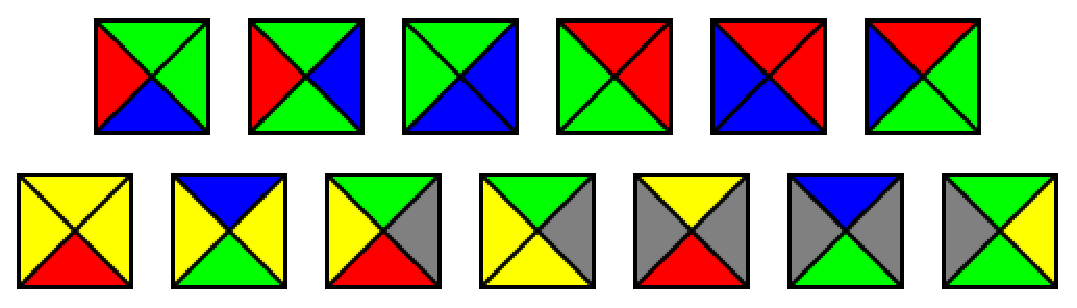
\includegraphics[scale=0.4]{wang13.eps} 
\caption{Smallest aperiodic wang tiles.}
\label{fig:wang13}
\end{figure}

The method of construction used is called expanding squares. It is based on the idea of superimposing a number of related things. Below we present one of the possible ways to encode fibonacci series.

\section*{Turing Machines}
A Turing machine is a formal way of describing computation. It is described as an abstract computer that has the capability of reading and writing symbols on tape extendable infinitely on atleast one side. The machine starts in a given state, and reads a symbol on the tape, and depending on the combination of symbol read and the state the machine is in, it may write a new symbol, and move forwards or backwords on the infinite tape.

We can simulate any Turing machine using Wang tiles by taking advantage of the fact that each Wang tile forces the arrangement of its neighbours. In particular we can treat a row of Wang tiles as the state of Turing machine tape at an instant of time. Since the state of Turing machine is determined completely by its past history, This construction gives us the ability to simulate each instant of a Turing machine in a single row. The same way that the next instant is forced on the turing machine by the state it is in, and the history of the machine, the next row is forced on the Wang tiles by the current row. In our examples we use the encoding of Turing machines into Wang tiles given by \cite{chaitin}.

The encoding can be understood as follows, The colours or sides of wang tiles correspond to a blank symbol (b), the symbols on the turing machine tape, turing machine states, and tuples of the form (tape symbols , internal state). We choose a unique colour or jagged edge for each possibility. We call each line in the tiling the next generation tape. I will use the tuple (left,up,down,right) as the notation for a single tile.

Next we formulate the wang tiles themselves. We need tiles that can transport inactive tiles directly to the next generation. For this, we need as many wang tiles of the form (b,symbol,symbol,b) forall tape symbols. This will ensure that any symbol on an inactive tile is moved to the next generation by default.

Next we need to simulate the movement of the read write head. In case the read write head doesn't move, this can be encoded in the tuple (b,(current state,symbol), (newstate,newsymbol), b). If the readwrite head moves left, then that can be encoded by forcing the left tile to change. (newstate,(newstate,newsymbol),newsymbol,b). If the head moves right, the tile needed is (b,(newstate,newsymbol),newsymbol,newstate). Once we have a new state as the right or left, then the right or left tile next to it also needs to have the same colour, and hence we can make that tile the location of the head. The movement of head to left is encoded by (b,symbol,(newsymbol,newstate),newstate). If it was moved right, then it would be (newstate,symbol,(newsymbol,newstate),b). Notice how we can always tell where the read write head is by looking for a tuple at the bottom of the tiles. At any point there would be atmost a single tuple at the bottom when we encode a turing machine this way.

We give below a few simulations of Turing machines using Wang tiles.

\section*{Related Work}
The original solution to Turing machine with Wang tiles was created using 20,426 tiles by Berger. It was later brought down to 104 by him, and later to just 13 tiles by Karel Culik \cite{culik}. Wang tiles are just one form of tiling. Another was discovered by Roger Penrose called Penrose tiling. Penrose tiling \cite{penrose} is a non-periodic self similar quasi crystal tiling of a plane, and the smallest number of tiles required for tiling a plane is just two. Another related field is cellular automata. These also produce very complex and often turing complete patterns with very simple rules \cite{wolfram}. One of the smallest cellular automata was proven recently to be turing complete \cite{cook}.

A few other applications of wang tiles include graphics texture generation \cite{texture}, Molecular self assembly \cite{assembly} and DNA computing \cite{dna}. Wang cubes \cite{cubes} the 3-D analog of Wang tiles have also been a field of research for its properties in video generation.

\section*{Simulation}
We modelled the Wang tiles using haskell, and used it to verify our constructions. Our model includes facilities to input the tilings used, the initial configuration and the constraining side tiles. 

\section*{Conclusion}
In this paper we explored wang tiles that are able to tile a plane aperiodically. For this we used two different techniques. The first was direct tiling as given in \cite{tilings}, and later by simulating a Turing machine on the Wang tiles as given in \cite{tmtiles}.

\bibliographystyle{apalike}   % (uses file "plain.bst")
\bibliography{wang}       % expects file "myrefs.bib"
\end{document}

